\documentclass[../Main.tex]{subfiles}

\begin{document}
\author{Current} %use author for title of lesson
\date{Year 1 Topic 12} %use date to refer to topic in main booklet

\section{Current} %Section is the title of the lesson repeated, ready for the main contents page.

\begin{frame}{Definitions}
    \begin{block}{Charge \textbf{Q}}
    Charge is a fundamental property that has units Coulombs. The charge of an electron is $1.6\times10^{-19}$C, important to know as \emph{electr}ons are usually the charge carriers for \emph{electr}icity.
    \end{block}
    {\small Interesting side note, electricity was named as a phenomenon \emph{before} the discovery of the electron}
    \pause
    \begin{block}{Current}
    Current is the rate of flow of charge - proportional to the number of charge carriers (usually electrons) flowing past a certain point per second. It has units Amperes/Amp (A) -- which is one of the SI units. \newline 
    \end{block}
    \pause
    \begin{equation*}
       \mbox{Current: } I = \frac{\Delta Q}{\Delta t}
    \end{equation*}
\end{frame}

\begin{frame}{Link between Charge and Current}
    The coulomb itself is defined by current. 
    \begin{block}{The Coulomb}
    1 Coulomb is defined as the amount of charge that flows in one second when the current is 1.0A.
    \end{block}
    
    {\large
    \begin{equation*}
        \Delta Q=I\Delta t
    \end{equation*}}
    
    How many electrons is this equivalent to? \pause
    -- $6.25\times 10^{18}$
    \pause
    \begin{block}{Charge as a +n}
    Charge can be represented as a number, e.g. +1 or -2 as the chemists may be familiar with -- but this in Physics is incorrect. Instead we would write this as +e or -2e, where \emph{e} is the \emph{elementary charge}. What might this be?
    \end{block}
\end{frame}

\begin{frame}{Examples}
    \begin{exampleblock}{Example}
    What is the current if 1 coulomb of charge passes a point in a wire in 0.8 seconds? \newline \pause
    1.25A
    \end{exampleblock}
    
    \pause
    -- Your turn. Kerboodle page 121.
\end{frame}

\begin{frame}{Conventional current}
    Before the electron was discovered, it was thought that the charge carrier in a circuit was a positive charge, going from + to -. \pause 
    With the discovery of the electron, it was realised that the electron as a negative charge comes from - to +.
    \newline \newline \pause
    Problem was everyone was used to the old way of thinking and didn't want to change so they named the two types `conventional current' and `electron flow/current'. We will take current to be conventional here, unless a question specifically states otherwise.
    
    \begin{figure}
        \centering
        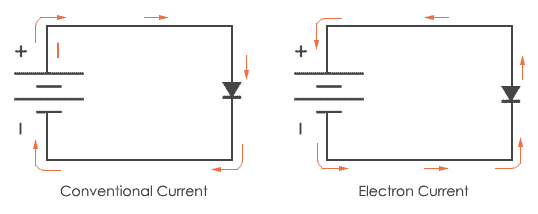
\includegraphics[height=3cm]{Electricity_Images/conventional_current.png}
    \end{figure}
\end{frame}

\begin{frame}{Current at junctions}
    At a junction in a circuit, the total current entering is equal to the current leaving. This is known as \emph{Kirchhoff's first law}. In other words, current merges and splits at a junction -- thinking about current as electrons moving, they don't disappear at all and must take one of the possible routes round the circuit
    \pause
    \begin{block}{Kirchhoff's First Law}
    For any junction in a circuit, the sum of the current in is equal to the sum of the currents leaving.
    \begin{equation*}
        \Sigma I_{in} = \Sigma I_{out}
    \end{equation*}
    \end{block}
    \pause
    Examples:
    \begin{figure}
        \centering
        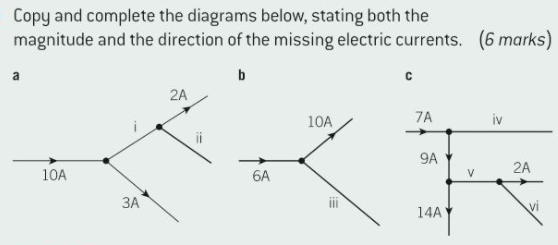
\includegraphics[height=2.5cm]{Electricity_Images/kerboodle_Qs.png}
    \end{figure}
\end{frame}

\begin{frame}{Drift Velocity}
\begin{multicols}{2}
    We can think of current as electrons (or some other charge carrier) moving through a circuit. But how fast do they actually move? Or in other words -- what is the speed of electricity? \pause
    \newline \newline
    The mean drift velocity gives you the velocity of the charge carrier in a circuit:
    \begin{equation*}
        I = Anev
    \end{equation*}
    \columnbreak
    \begin{figure}
        \centering
        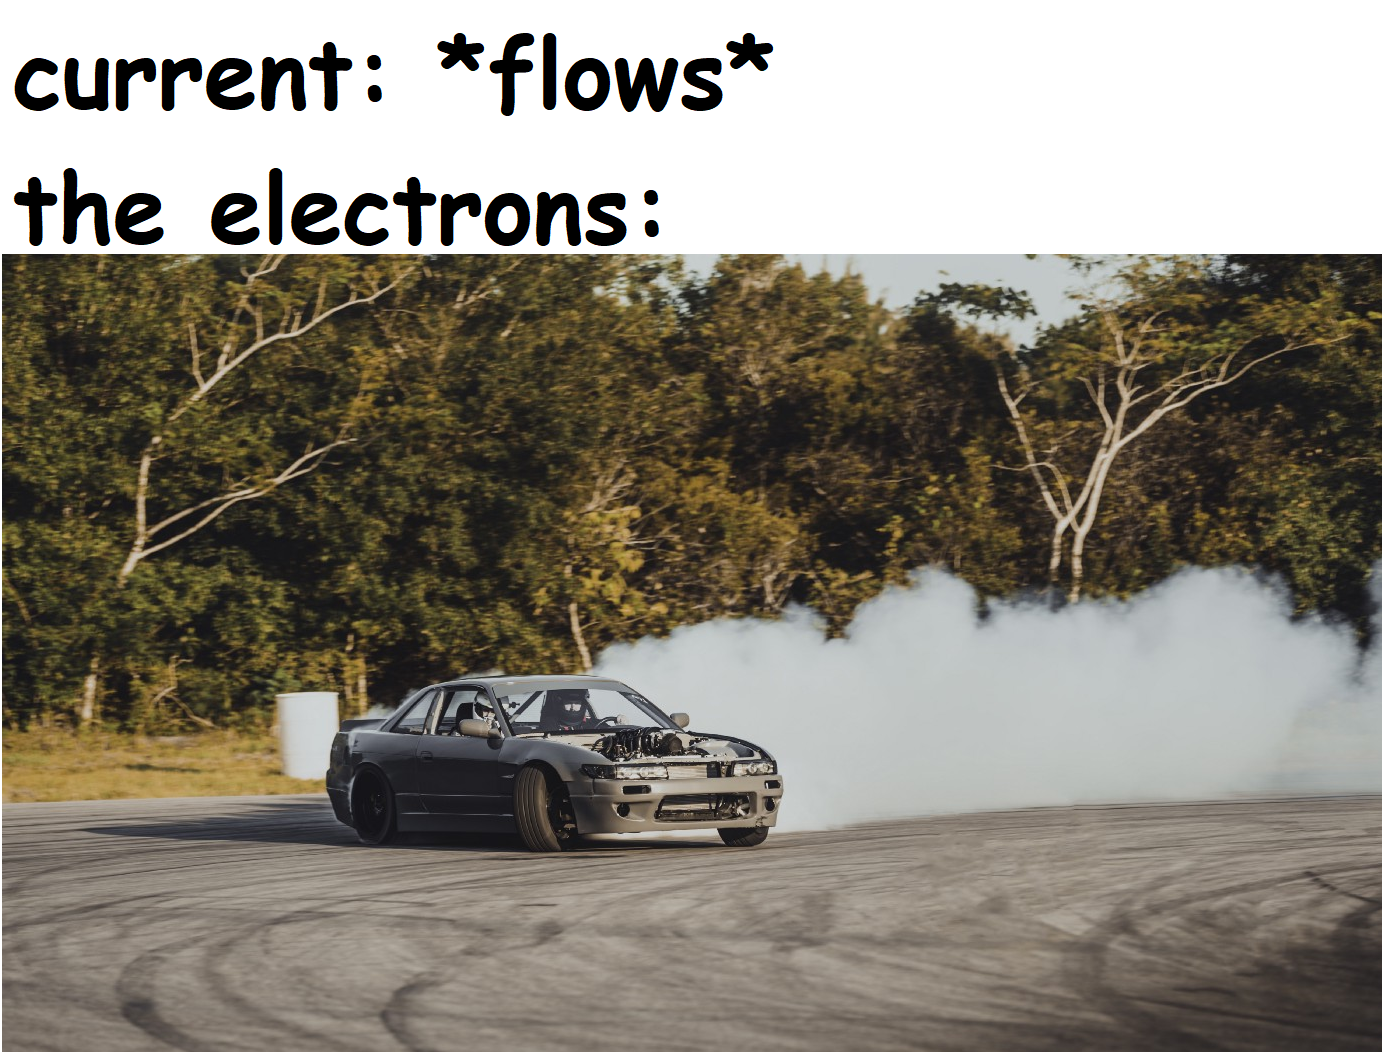
\includegraphics[width=5cm]{Electricity_Images/drift_velocity_meme.png}
    \end{figure}
    \end{multicols}
    \begin{multicols}{2}
    {\small where:
    \begin{itemize}
        \item I is the current in Amps. 
        \item A is the cross-sectional area of a wire
    \columnbreak
        \item n is the number density of electrons -- in units $m^{-3}$
        \item e is the charge of the electron
        \item v is the drift velocity in $ms^{-1}$
    \end{itemize}}
    \end{multicols}
\end{frame}

\begin{frame}{Changing the wire}
    What might happen to the drift velocity if the diameter of a wire changes part way? -- why? 
    \pause
    \begin{figure}
        \centering
        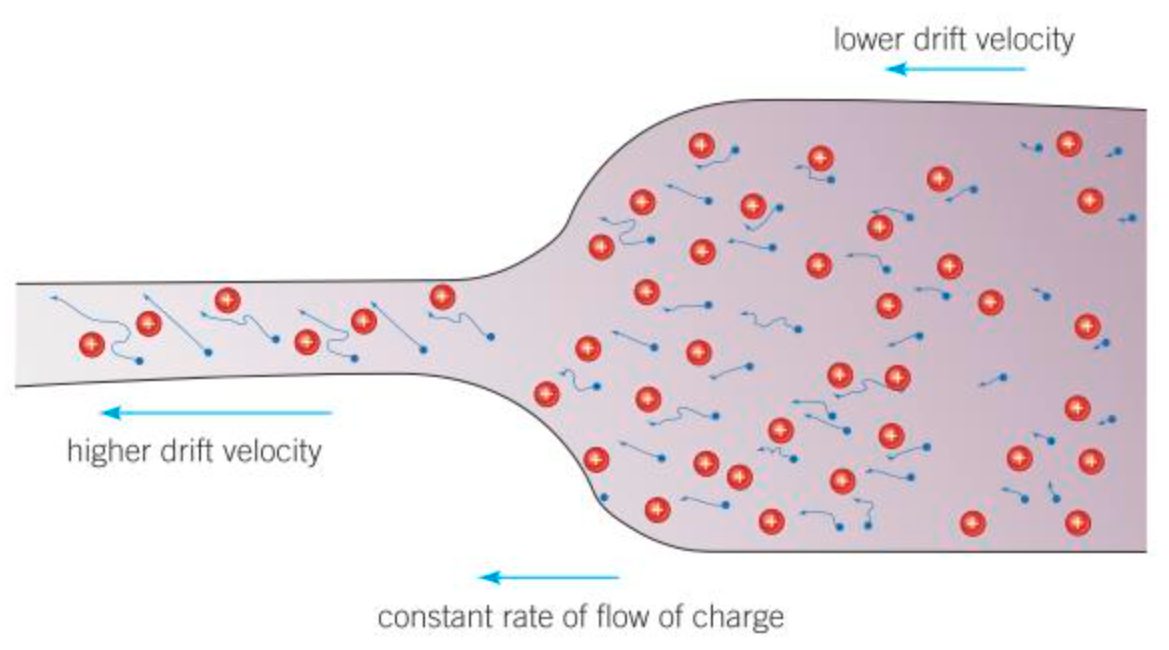
\includegraphics[height=2.4cm]{Electricity_Images/changing_wire.png}
    \end{figure}
    
    \begin{exampleblock}{Example}
    A copper wire has a diameter of 2mm. The number density of copper is $8.5\times10^{28} m^{-3}$. Calculate the mean drift velocity of the electrons through the wire when the current is 1.40A. \pause
    -- $3.28\times 10^{-5}ms^{-1}$ \newline \pause
    
    Without calculation, compare this to the mean drift velocity if the diameter is now 1.2mm and we keep the same current. \pause
    -- it is now faster, by a factor of $\frac{2^2}{1.2^2}=\frac{25}{9}$, as $v\propto \frac{1}{A}, A\propto d^2$
    \end{exampleblock}
\end{frame}

\begin{frame}{Conductors vs Insulators}
\begin{multicols}{2}
    Everything we have looked at today assumes we have some sort of conductor -- that is to say, a material that allows current to flow. 
    \newline \newline
    But how could we define a conductor, and what makes a good conductor? 
    \pause
    \begin{figure}
        \centering
        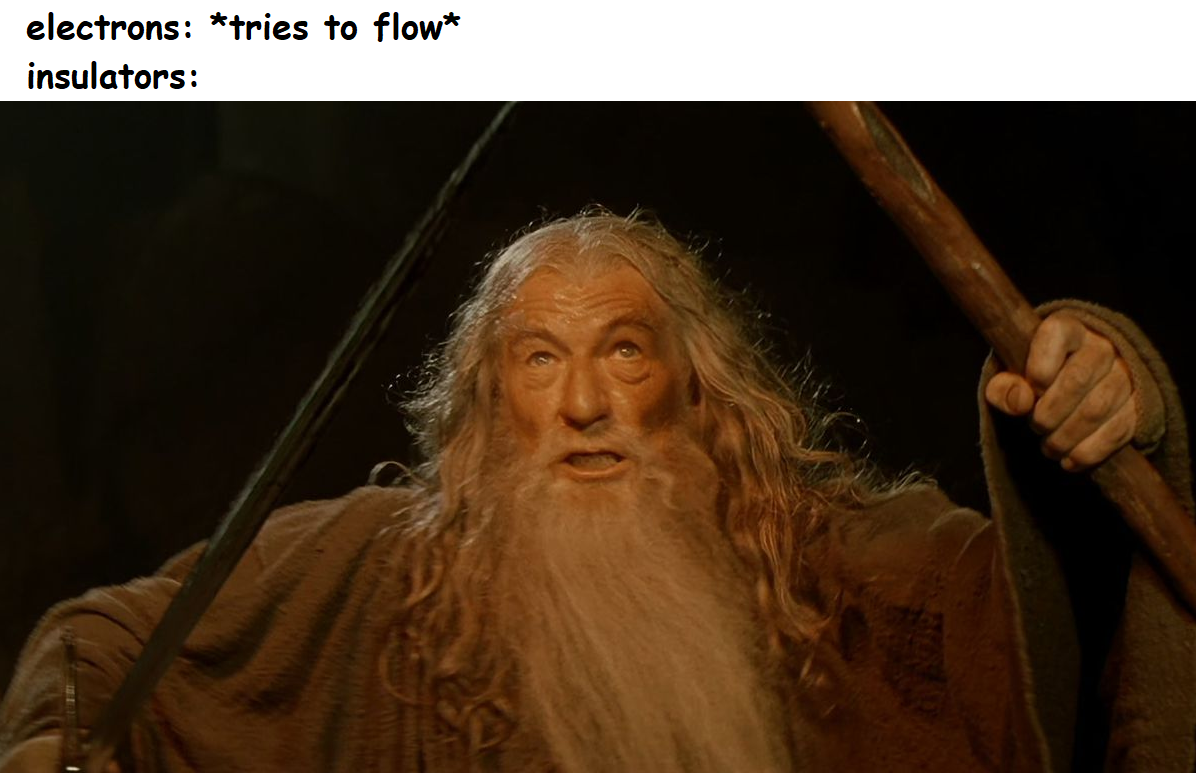
\includegraphics[height=3cm]{Electricity_Images/you_shall_not_pass.png}
    \end{figure}
    \end{multicols}
    
    \begin{block}{Conductors vs Insulators}
    A conductor is a material that has a lot of free electrons, and thus a high number density on the order of $10^{28} m^{-3}$. An insulator is the opposite with a very low -- or even zero -- number density. Between the two, typically on the order of $10^{17} m^{-3}$ are semi-conductors, which we will see in the coming weeks.
    \end{block}
    
\end{frame}

\end{document}